
\section{Appendix}

\subsection{Grid cell module}

It is defined a correspondence between the global environment in which the agent moves, a two-dimensional Euclidean space $\mathbf{R}^{2}$, and a bounded local space of a grid module, corresponding to a torus.

The global velocity $\mathbf{v}=\{x,y\}$ is then mapped to a local velocity, scaled by a speed scalar $s^{\text{gc}}_{l}$ specific to the grid cell module $l$, which determines its periodicity in space.

The choice of a toroidal space is motivated by consolidated experimental evidence of the neural space of grid cells, which are organized in modules of different sizes spanning the animal's environment. However, the shape of their firing pattern is known to be hexagonal, which corresponds to the optimal tiling of a two-dimensional plane, giving rise to a neural space lying on a twisted torus.
In this work, for simplicity, we consider a square tiling and thus a square torus, without much loss of generality except for the slight increase of grid cells required for a sufficiently cover.

A grid cell module $l$ of size $N^{\text{gc}}$ is identified by a set of positions defined over a square centered on the origin and size of $2$, such that $\{(x_{i}, y_{i})\;\vert\; i \in N^{\text{gc}}\;\land\;x_{i},y_{i}\in (-1, 1)\}$.
This local square space has boundary conditions for each dimension, such that, for instance, when $x_{t} + s^{\text{gc}}_{l} \cdot v_{x} > 2$ the position update is taken to the other side $x_{t+1} = x_{t} + s^{\text{gc}}_{l} \cdot v_{x} - 2$, where $s^{\text{gc}}_{l}$ is the scale of the velocity in the local space of the module $l$ with respect to the real global agent velocity $v=\{v_{x}, v_{y}\}$.
When the module is initialized, the starting positions of its cells are uniformly distributed over the square forming a lattice.
When the agent is reset in a new position at the beginning of new trial, a displacement vector is applied to the last cells positions such that the mapping between the module local space and the global environment is preserved.

The firing rate vector of each cell is determined with respect to a 2D Gaussian tuning curve centered at the origin at $(0,0)$, and it is calculated as \\ $r_{i} = \exp\left(-\frac{x^{2}_{i} + y^{2}_{i}}{\sigma^{\text{gc}}_{l}}\right)$, where $\sigma^{\text{gc}}_{l}$ is the width of the tuning curve for module $l$.
An illustration of the receptive field over a 2D environment and a toroidal space is reported in Figure \ref{fig:gridpc}\textbf{a}-\textbf{b}.

The final population vector of the grid cell network GC is the concatenated and flattened firing rate vector of all modules $\textbf{u}^{\text{GC}}$.

\hfill \break
In our model, each grid cell had a tuning width of 0.04. They were defined as 8 modules of size 36, and the relative speed scales were $\{1., 0.8, 0.7, 0.5, 0.4, 0.3, 0.2, 0.1, 0.07\}$.

\subsection{Place cells}

\paragraph{Tuning formation}
% formation | forward + competition
The tuning of a new place cell is simply defined as the current GC population vector $\textbf{u}^{\text{GC}}_{t}$, and its index is that of the first silent cell, which is added to the forward weight matrix $\textbf{W}_{i}^{\text{GC}to \text{PC}}\leftarrow \textbf{u}^{\text{GC}}$.

In order to avoid overlapping of place fields, lateral inhibition is implemented. More specifically, the tuning process is aborted in case the cosine similarity of the new pattern and the old ones is greater than a threshold $\theta^{\text{PC}}_{\text{inh}}$.

Each cell represents a position in the GC activity space, which can be considered a node within a graph of place cells (PC).
Although it is totally possible to only use the $N^{\text{GC}}$-dimensional tuning patterns and be agnostic about the dimensionality of the space in which the agent lives, to simplify the calculations, we mapped each pattern to 2D positions in a vector space.
Then, the PC recurrent connectivity matrix is calculated with a nearest neighbors algorithm, which instead of a fixed number $K$ of neighbors uses a lateral distance threshold $\theta^{\text{PC}}_{\text{rec}}$.

\paragraph{Activity} The current firing rate of the PC population is determined by the cosine similarity between the GC input and the forward weight matrix, then passed through a generalized sigmoid $\phi(z)=\left[1 + \exp(-\beta(z-\alpha))\right]^{-1}$.
The parameter $\alpha$ represents the activation threshold, or horizontal offset, while $\beta$ the gain, or steepness.

\begin{equation}
    u^{\text{PC}}_{i}=\phi\left(\cos\left(\textbf{u}^{\text{GC}},\textbf{W}^{\text{GC},\text{PC}}_{i}\right)\right)
\end{equation}

It is also defined as an activity trace, which has an upper value of 1 and decays exponentially:

\begin{equation}
    m_{i} = - m_{i} / \tau^{\text{PC}} + u_{i}
\end{equation}

\noindent It is used as a proxy for a memory trace.

\hfill \break
In the model, a PC population is defined by its average place field size, determining the granularity of the representation of the place.
In plot \ref{fig:gridpc}\textbf{b} it is illustrated an example of place cells layer tuning obtained from a continuous trajectory over a square environment.

\begin{figure}[ht]
    \centering
    \includegraphics[width=1.\textwidth]{figures/pc_gc.png}
    \caption{\textbf{Place fields obtained from grid cells activity} - \textbf{a}: \textit{grid cell modules with different granularity represented over a continuous trajectory in an open space. For visualization purposes, each module is represented as composed of four sub-modules of 9 grid cells each, whose periodic tuning generates activity that repeats
    in space}.
    \textbf{b}: \textit{place cells whose spatial tuning has been obtained from the concatenation of the grid cells population vector.}}
    \label{fig:gridpc}
\end{figure}


\subsection{Modulation}

Neuromodulation is implemented as a reward-sensitive signal, represented as DA (mimicking the function of dopamine), and a collision-sensitive signal, represented as BND (for boundary).
Its dynamics are defined in terms of a leaky variable $v$ whose state is perturbed by an external input $x$, whose qualitative meaning differs for each neuromodulator $k$.

\begin{equation}
\begin{aligned}
    v^{k} &= - v^{k} / \tau^{k} + x^{k} \\
    v^{k} &= \text{max}(v^{k}, 0)
\end{aligned}
\end{equation}

$\tau_{\text{DA}}=2,\,\tau^{\text{BND}}=1$

% plasticity
\paragraph{Learning rule}
The connection weights $\textbf{W}^{k}$ are updated according to a plasticity rule composed of an Hebbian term, involving the leaky variable, the place cells that are above a certain threshold $\theta^{k}$, and the current connection weights value:

\begin{equation}
    \Delta \mathbf{W}^k = \eta^k \mathbf{u}^{\text{PC}} \left(v^k - \mathbf{W}^{k}\right)
\end{equation}

\noindent where the weight contribution of the Hebbian update, and $\eta^{k}$ is the learning rate: $\eta^{\text{DA}}=0.9,\,\eta^{\text{BND}}=0.9$.
Additionally, connections values are kept non-negative.

\paragraph{Active neuronal modulation}
Neuromodulation acts on the neuronal profile of the place cells by affecting the value of the activation gain and relocate the center of their tuning.

Gain modulation is implemented using the activity traces and a constant reference gain value $\bar{\beta}$:
\begin{equation}
    \beta_{i} = c^{k}_{a} m_{i} \bar{\beta} + (1 - m_{i}) \bar{\beta}
\end{equation}

\noindent where $c^{k}_{a}$ is a scaling gain parameter, and if it is 1 then no modulation takes place.

% remapping
Concerning center relocation, it is applied to recently active neurons with non-zero trace $m_{i}$.
For a place cell $i$ with position $\textbf{W}^{\text{GC,PC}}_{i}$ (in the grid cell space), it is calculated a displacement vector $q_{i}$ with respect to the current position $\textbf{u}^{\text{GC}}$:

\begin{equation}
    q_{i} = c^{k}_{b} v^{k} \exp\left(-\frac{\|\textbf{W}^{\text{GC,PC}}_{i}-\textbf{u}^{\text{GC}}\|}{\sigma^{k}}\right)
\end{equation}


\noindent where $c^{k}_{b}$ is a scaling relocation parameter, while $\sigma^{k}$ the width of the Gaussian distance.
This displacemented is used to move in GC activity space and get the new GC population vector to use as tuning pattern.

Also in this case, it is ensured that the new place field center is at a minimum distance $\theta^{PC}_{\text{min}}$ from the others; here Euclidean distance is used.


\subsection{Decision making}

\paragraph{Behaviour selection logic}
\hfill \break
The possible behaviours are \textit{exploration} and \textit{exploitation}, and an action is defined as a 2D velocity vector.
For exploration, an action can be generated either as random navigation, using a polar vector of fixed magnitude (the speed) and angle sampled from a uniform distribution, or as a step within a goal-directed navigation plan to reach a random destination, which corresponds to a randomly sampled existing place cells.
In the goal-directed navigation the magnitude of the velocity vector is less or equal than a fixed speed value, depending on the distance from the next target position in the plan
Instead, for the exploitation behaviour, the action is a step within a goal-directed navigation towards the reward location.
The behaviour selection process depends on the experience of collision, the presence of a plan, and the success in the navigation planning. A diagram of this logic is reported in Figure \ref{fig:dm_logic}.

\begin{figure}[h]
    \centering
    \includegraphics[width=0.7\textwidth]{figures/pcnn_dm_logic.png}
    \caption{\textbf{Diagram of the behaviour selection process}}
    \label{fig:dm_logic}
\end{figure}

\noindent The positions of the agent and of the target location for planning are identified by the place cells population vector.
In particular, the reward position $(x_{r}, y_{r}$ is determined by the weighted average of the centers $x_{i}, y_{i}$ of the place cells with respect to their DA-modulated connections weights. Further, only the top 5 place cells are considered.

\begin{equation}
    \begin{aligned}
        x_{r} &= \sum\limits^{5}_{i} \textbf{W}^{DA}_{i} x_{i} \\
        y_{r} &= \sum\limits^{5}_{i} \textbf{W}^{DA}_{i} y_{i} \\
    \end{aligned}
\end{equation}


\paragraph{Path-planning algorithm}
\hfill \break

\begin{algorithm}[H]
    \caption{\textsc{Activity-based Pathfinding}}
\begin{algorithmic}[1]
\Require Connectivity matrix $C \in \mathbb{R}^{n \times n}$, node weights $w \in \mathbb{R}^n$, start node $s$, end node $e$
\Ensure A list of nodes forming a (short) path from $s$ to $e$, or empty if none found
\State Initialize activity vector $a \gets \mathbf{0} \in \mathbb{R}^n$; set $a_s \gets 1$
\State Initialize history list $H \gets [\,]$
\Comment{\textit{--- Forward propagation phase ---}}
\For{$t = 1$ to \texttt{MAX\_PATH\_DEPTH}}
    \State $a \gets C \cdot a$
    \State $a \gets a \circ w$ \Comment{Element-wise multiplication with node weights}
    \State $a \gets \sigma(4(a - 0.6))$ \Comment{Apply sigmoidal activation: $\sigma(x) = \frac{1}{1 + e^{-x}}$}
    \State $a_i \gets 0$ if $a_i < 0.1$ (thresholding)
    \State Append $a$ to $H$
    \If{$a_e > 0$}
        \State \textbf{break}
    \EndIf
\EndFor
\If{maximum depth reached}
    \State \Return $[\,]$ \Comment{No path found}
\EndIf
\If{$|H| < 3$}
    \State \Return $[s, e]$ \Comment{Path is trivially short}
\EndIf
\Comment{\textit{--- Backward traceback phase ---}}
\State Initialize path index stack $G \gets [[e]]$
\For{$t = 1$ to \texttt{MAX\_PATH\_DEPTH}}
    \State Let $m \gets C_{G[t-1]}$ \Comment{Get neighbors of current group}
    \If{$m_s > 0$}
        \State \textbf{break}
    \EndIf
    \State $a \gets H[-(t+1)] \circ m$
    \State Append $\{i : a_i > 0\}$ to $G$
\EndFor
\Comment{\textit{--- Path reconstruction ---}}
\State $P \gets [e]$
\For{$t = 1$ to $|G| - 1$}
    \State Initialize $a \gets \mathbf{0} \in \mathbb{R}^n$
    \State Set $a_i \gets 1$ for all $i \in G[t]$
    \State $a \gets a \circ C_{P[-1]}$
    \If{$\sum a = 0$}
        \State \Return $[\,]$ \Comment{No valid neighbor}
    \Else
        \State Choose $j \in \{i : a_i > 0\}$ uniformly at random
        \State Append $j$ to $P$
    \EndIf
\EndFor
\State Append $s$ to $P$
\State \Return $\text{reverse}(P)$
\end{algorithmic}
\end{algorithm}\label{alg:pathalg}

% policy algorithm

% result figure
The planning of a new route is implemented as a path-finding algorithm based on the place cell graph, provided as connectivity matrix $C$.
Its particularity is the use of a weighting $\widetilde{\textbf{W}}$ of the nodes according to the neuromodulation map. A description is reported in algorithm \ref{alg:pathalg}.


\subsection{Environments}

The game in which test the model has been developed with the python library Pygame, used under license GNU LGPL version 2.1 and available at \url{https://github.com/pygame/pygame}.
The environment layout consisting in a customizable arrangement of vertical and horizontal hard walls with variable length and fixed width. Below in Figure \ref{fig:rooms} some samples are shown.

\begin{figure}[H]
    \centering
    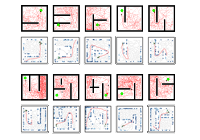
\includegraphics[width=0.9\textwidth]{figures/maps_envs.png}
    \caption{\textbf{Sample of generated environments}}
    \label{fig:rooms}
\end{figure}

The reward object is defined as a circle with size the 5\% of the total environment area.
When the agent position is within its boundary, it is provided a binary signal $R\sim \mathcal{B}(p_{r})$ drawn from a Bernoulli with probability $p_{r}=0.6$.
The duration of the reward fetching is set to 2 time steps.

The agent object is defined as a square with size the 3.3\% of the total environment area.

The testing protocol was inspired by the behavior of animals that venture into new territories in search of food. It was divided into two parts:
\begin{itemize}
    \item \textbf{exploration phase}: the agent was placed in a random location within the environment for 10'000 time steps.
        In this phase the reward is not present.
        Further, in order to force greater exploration of the environment, every 3'000 steps it was teleported to another random location. This external intervention was meant to mitigate the randomness in the exploratory behavioural strategy of the agent.

    \item \textbf{reward phase}: a reward is insert in a random location, and it is available to be discovered. When it is encountered, the agent is teleported to a random location within the environement, and after a fixed about \~100 time step it is enabled its reward-seeking behaviour, in
        the form of goal-directed navigation.
        The total duration of this phase is set to 20'000 time steps.

\end{itemize}

An episode is defined as a continuous trajectory during the reward phase, namely a set of time steps starting from when the agent is place in a position until either it finds the reward or the simulation ends.

\paragraph{Detour experiment}
The protocol is modified such that after a fixed number of episodes the layout of the environment is changed, \textit{e.g.} a wall is inserted.
This experiment is meant to test the ability to reach the reward location by using the same cognitive map, and possibly update it with the new sensory information, such as the detection of the new boundaries. 

\paragraph{Changing reward experiment}
During the reward phase, the reward location is changed after a fixed number of fetches.

\paragraph{Optimization}
The model hyper-parameters such as the constants for the neural dynamics and the behaviour selection have been optimized through a evolutionary algorithm.
Initally, an initial population of individuals with different random genomes (string of hyper-parameters values) is evaluated according to a fitness function, in this case a set of different environments. \\
Next, the population of a new generation is constructed from the first by combining and mutating the genomes of the top ranked individuals from the previous generation. \\
In particular, we used the Covariance Matrix Adaptation algorithm, in which the shape of distribution of genome values is iteratively adapted according to the recent performances.

The evolved hyper-parameters are: neural gain $\beta$, lateral inhibition threshold $\theta^{\text{PC}}_{\text{inh}}$, lateral distance threshold $\theta^{\text{PC}}_{\text{rec}}$, activity trace time constant $\tau^{\text{PC}}$, reward modulation scale $c^{\text{DA}}_{b}$, reward modulation spread
$x^{\text{DA}}_{b}$, boundary modulation scale $c^{\text{BND}}_{b}$, boundary modulation spread $c^{\text{BND}}_{b}$, reward gain modulation $c^{\text{DA}}_{a}$, and boundary gain modulation $c^{\text{BND}}_{a}$.
The distribution of the genome values is reported in Figure \ref{fig:evoplot}.

\begin{figure}[ht]
    \centering
    \includegraphics[width=1.\textwidth]{figures/evoplot.png}
    \caption{\textbf{Distribution of evolved parameters} - \textit{Results relative to the last generation, from a run with population size of 128 individuals.}}
    \label{fig:evoplot}
\end{figure}

